\documentclass{beamer}
\mode<presentation> {
  \usetheme{Darmstadt}
}

\usepackage{graphicx} 
\usepackage{booktabs}


\title[2023-2024]{Simple Modeling of Road Traffic.} 

\author{Gerbaud Florent \\ Fatima Rharrour \\ MAM4} 
\institute[Polytech Nice-Sophia] % Your institution as it will appear on the bottom of every slide, may be shorthand to save space
{
Supervisor: \\ % Your institution for the title page
\medskip
{Didier Auroux} % Your email address
}
\date{\today} % Date, can be changed to a custom date
\titlegraphic{
\includegraphics[width=3cm]{Polytech.png}} %
%-----------------------------------------------------------------------------------------
\AtBeginSection[]
{
	\begin{frame}
		\frametitle{Table of Contents}
		\tableofcontents[currentsection]
	\end{frame}
}
\begin{document}

\begin{frame}
\titlepage 
\end{frame}

\begin{frame}
\frametitle{Table of contents} 
\tableofcontents
\end{frame}

%----------------------------------------------------------------------------------------
%	PRESENTATION SLIDES
%----------------------------------------------------------------------------------------

%------------------------------------------------
\section{Introduction:} 
%------------------------------------------------
\begin{frame}
	\begin{center}
		\frametitle{What is Road Traffic Modelling?}
	\end{center}
	\begin{columns}
		\column{0.6\textwidth}
		\begin{itemize}
			\item Representing complex dynamics of vehicles moving along roads.
			\item Creating mathematical and computer models for:
			\begin{itemize}
				\item Understanding vehicle flow.
				\item Predicting movement patterns.
				\item Analyzing interactions on roads and highways.
			\end{itemize}
		\end{itemize}
		
		\column{0.4\textwidth}
		\begin{center}
			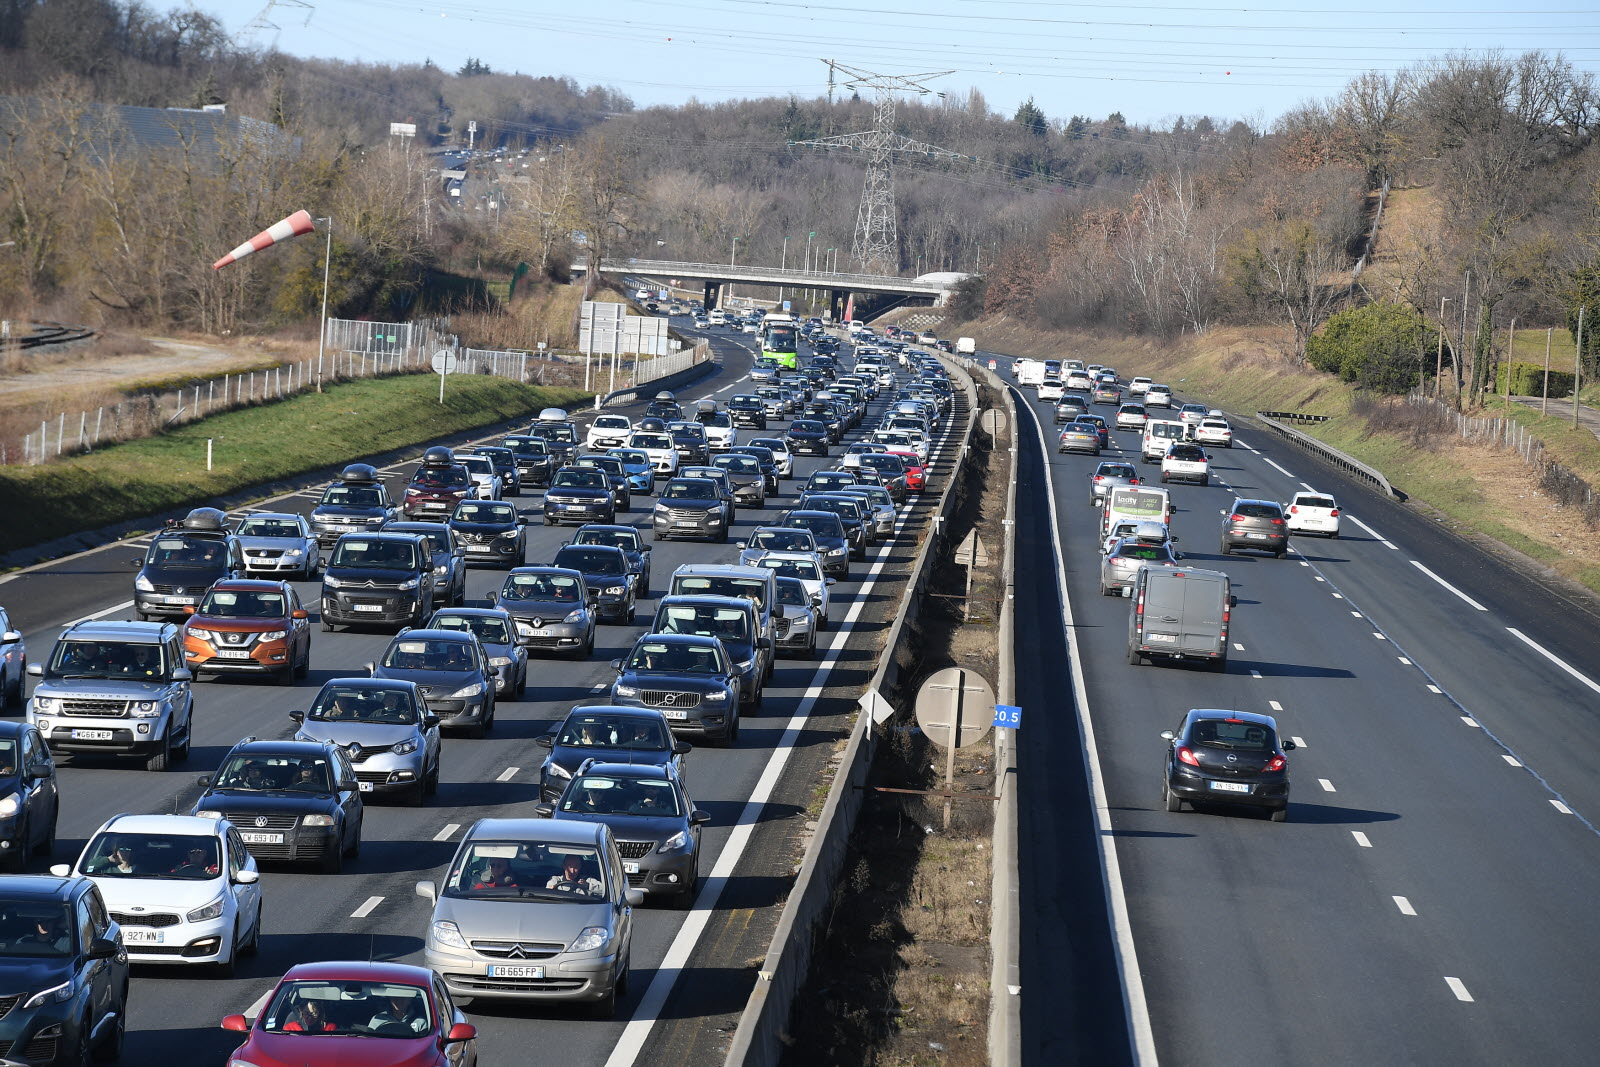
\includegraphics[width=\textwidth]{PIC1.jpg}
			\tiny{\textit{Fig. 1: Real-life Road Traffic}}
		\end{center}
	\end{columns}
\end{frame}

%******************************************************************************************
\begin{frame}
        \frametitle{Presentation of the subject:}
	\begin{block}{Key Benefits of Road Traffic Modeling}
		\begin{itemize}
	\item \textbf{Avoiding Traffic Jams:} Helps find solutions to prevent traffic jams on roads.
	\item \textbf{Making Roads Better:} Finds ways to improve roads and make them work smoother.
	\item \textbf{Understanding How Traffic Works:} Helps figure out how different things affect traffic and predict what might happen.
	\item \textbf{Making Transportation Better:} Shows how well transportation works and helps make it even better.
	\item \textbf{Saving Time and Money:} Aims to reduce time spent waiting in traffic and the money spent on each trip.
\end{itemize}
	\end{block}
\end{frame}
%******************************************************************************************
\begin{frame}{Presentation of the subject}
    Animation à ajouter ??
\end{frame}
%******************************************************************************************
\begin{frame}
\subsection{Project Organization Overview}
\frametitle{Project Organization Overview}
\begin{center}
    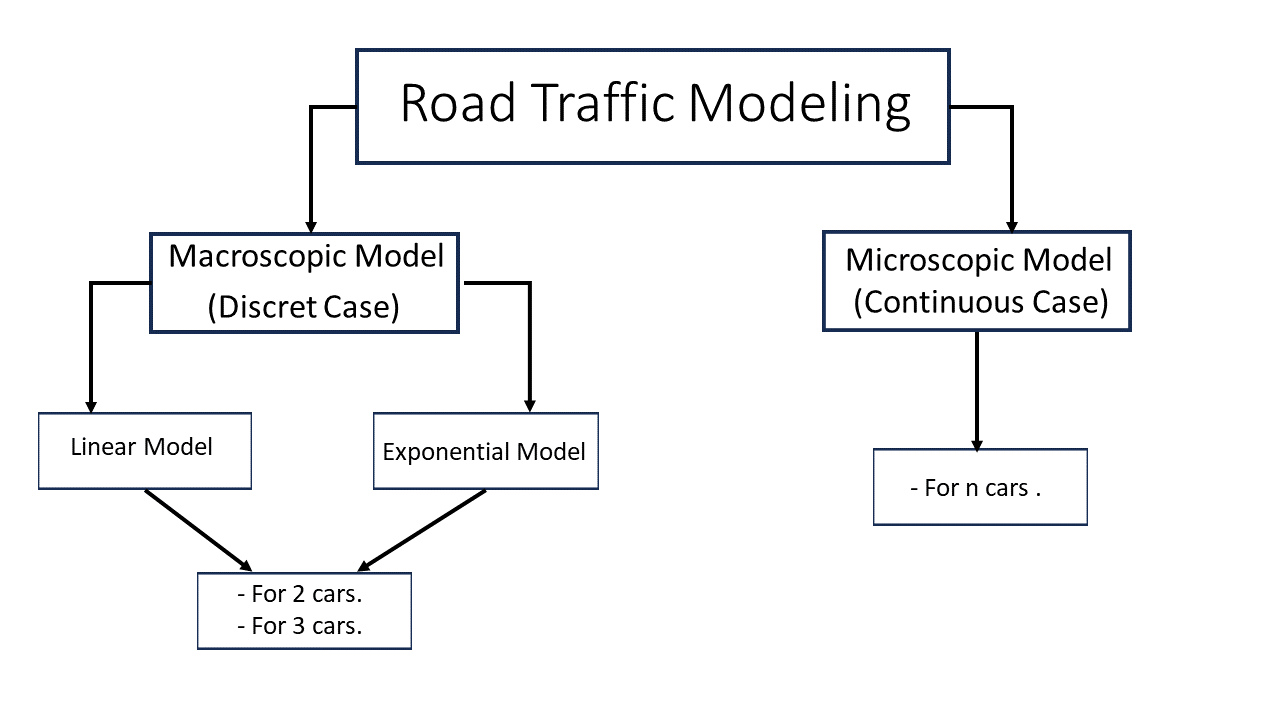
\includegraphics[width=1\textwidth]{org1.png} 
    \end{center}
\end{frame}
%******************************************************************************************
\begin{frame}{Useful Definitions}
	\vspace{-0.2cm}
	\begin{block}{Microscopic simulation}
		Microscopic simulation is a computer-based modeling technique that simulates the behavior of individual entities, such as vehicles or pedestrians, within a system
	\end{block}
	\vspace{-0.2cm}
	\begin{block}{Macroscopic simulation}
		Macroscopic simulation models systems at a higher, aggregated level, considering overall behaviors like traffic flow without detailing individual movements.
	\end{block}
	\vspace{-0.2cm}
	\begin{block}{Ordinary Differential Equation}
		An ODE is a mathematical equation that relates a function to its derivatives with respect to one or more independent variables.
		\[
		F\left(x,y,y',\ldots ,y^{(n-1)}\right)=y^{(n)}
		\]
	\end{block}
\end{frame}

%------------------------------------------------
\section{Study of the Discret Cas:}
%------------------------------------------------

\begin{frame}
\subsection{Differential Ordinary Equation:}
\frametitle{Differential Ordinary Equation (Theory):}
\begin{figure}
    \centering
    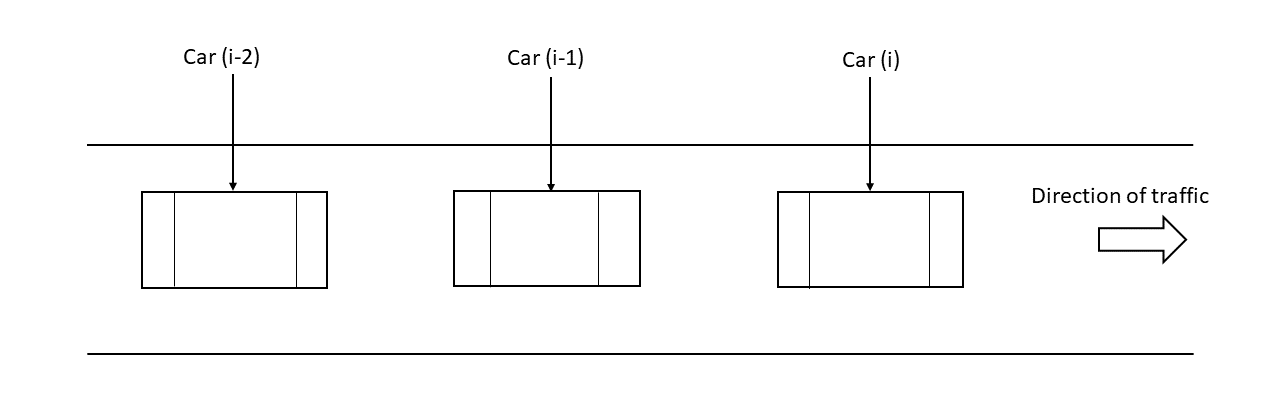
\includegraphics[width=0.6\textwidth]{discret.png} 
    \caption{ Discret Model.}
\end{figure}
    \begin{itemize}
			\item EDO to solve: $\boxed{y'(t) = f{\bigl (}t, y(t){\bigr )}}$.
			\item First step of the resolution: $\boxed{y_0 = y(t_0)}$.
			\item Recursive process to find the n-th solution of the EDO: $\boxed{y_{n+1} = y_{n} + hf(t_{n}, y_{n})}$
		\end{itemize}
\end{frame}

\begin{frame}
\subsection{Linear Model to represent velocity:}
\frametitle{Linear Model to represent velocity:}
Each car's movement is governed by a basic equation:
			
			\begin{align*}
				\dot{x_i}(t) = V_i = \alpha_i(x_{i-1} - x_i)
			\end{align*}
\newline
The system of equations for different cars is: 
    \begin{align*}
				\left\{
				\begin{array}{ll}
					\dot{x}_1 &= V_1 \\
					\dot{x}_2(t) &= \alpha_2(x_1 - x_2) \\
					&\vdots \\
					\dot{x}_n(t) &= \alpha_n(x_{n-1} - x_n)
				\end{array}
				\right.
			\end{align*}
\end{frame}
\subsubsection{Case of two cars:}  
\begin{frame}
\end{frame}
%------------------------------------------------
\subsubsection{Case of three cars:}  

\subsection{Special Model to represent velocity:}
%Cas des 3 voitures !!
\subsection{Study of Equilibrium and Stability}
\subsubsection{Using linear model:}
\subsubsection{Using the special model}
\section{Study of the continuous model:}
\begin{frame}{Mathematical Theory}
	\begin{alertblock}{Conservation Law}
		\begin{itemize}
			\item $\partial_t\rho + \partial_x\left[ \rho\left( 1-\frac{\rho}{\rho_{\text{max}}}\right) \cdot V_{\text{max}}\right] = 0 $
		\end{itemize}
	\end{alertblock}
	\begin{block}{Initial and Boundary Conditions}
		\begin{itemize}
			\item $\rho(x,0) = \rho_0(x), \quad x \in \Omega,$
			\item $\rho(0,t) = \rho(L,t), \quad t \geq 0$
			\item $\Omega := \left] 0,L\right[, $
			\item $\rho(x,t)$ represents the traffic density at position $x$ and time $t$, 
			\item $F(\rho)$ denotes the traffic flux as a function of density,
			\item $F(\rho)$ is often represented by a function modeling the relationship between traffic density and traffic velocity,
			\item $F(\rho) = V(\rho) \cdot \rho,$ where $V(\rho)$ is the traffic velocity as a function of density.
		\end{itemize}
	\end{block}
\end{frame}

\section{Euler Explicit Method}
\begin{frame}{Numerical Scheme for the resolution}
	\begin{alertblock}{Numerical Scheme}
		\begin{itemize}
			\item $\rho_{i}^{n+1} = \rho_i^n - \frac{\Delta t}{\Delta x} \cdot \left(\rho_i^n \cdot v_i^n - \rho_{i-1}^n \cdot v_{i-1}^n \right)
					=0$
		
			\item $v_i^n = \left( 1 - \frac{\rho_i^n}{\rho_{max}}\right)  \times V_{max}$
		\end{itemize}
	\end{alertblock}
	enrichir la slide. Peut etre ajouter le modèle dans la théorie et dire que quand on l'applique on obtient ca ou alors mettre une iage qui explique le shéma de Euler explicit ? 

	%slide : 
%Partie Math EDP
%Equation + cond au bord
%petite def de ce qu’il y a dans l’équation
\end{frame}

\begin{frame}
	\begin{figure}[H]
		\centering
		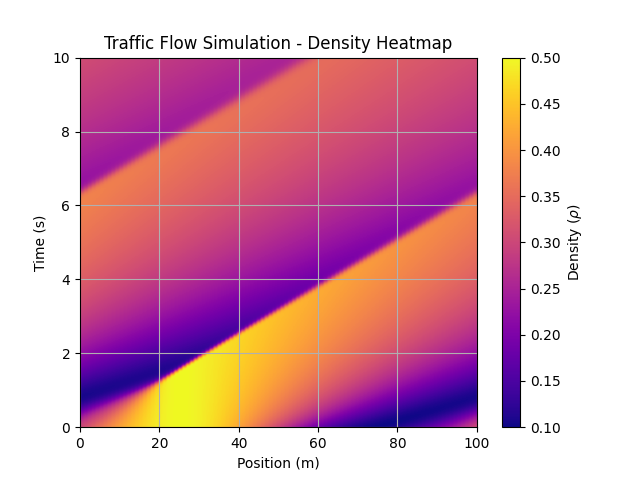
\includegraphics[width=0.65\textwidth]{traffic_flow_density_map.png}
		\caption[Traffic Flow Simulation With Euler Explicit]{\textbf{\underline{Traffic Flow Simulation With Euler Explicit:}} This figure illustrates the solution of the PDE at any time and position. Here is the link to the associated animation showing the movement of the traffic flow: \href{https://github.com/FlorentGerbaud/Simple-road-traffic-modeling/blob/Flo-PDE/SRTM/EDPMethod/CasTestToLaunch/TestToLaunch/Modele_IC_S/EulerExplicit/traffic_flow_animation.gif}{\textbf{\underline{Traffic Flow Simulation}}} }
		\label{fig:traffic_flow_density_map}
	\end{figure}
\end{frame}

\section{Conclusion}

\end{document}